% ============================================================
% Question Bank: ch06-06 Angle Relationships (Modified)
% Topic Title: Angle Relationships with Congruence, Similarity, and Multi-Step Problems
% CCSS: 7.G.B.5 (Modified for Virginia)
% Questions: 27 (15 MC + 6 SA + 6 Graphical)
% ============================================================

% --- Multiple Choice Questions (15) ---

\begin{practiceQuestion}{m-6-6-q01}{mc}
\begin{questionText}
Two supplementary angles measure $(4x + 12)°$ and $(2x + 48)°$. What is the value of $x$?
\end{questionText}
\choiceA{$15$}
\choiceB{$20$}
\choiceC{$24$}
\choiceD{$30$}
\correctAnswer{B}
\explanation{Supplementary angles sum to $180°$: $(4x + 12) + (2x + 48) = 180$. Combine: $6x + 60 = 180$. Subtract $60$: $6x = 120$. Divide: $x = 20$.}
\end{practiceQuestion}

\begin{practiceQuestion}{m-6-6-q02}{mc}
\begin{questionText}
Two complementary angles are $(3x - 7)°$ and $(x + 13)°$. What is the measure of the smaller angle?
\end{questionText}
\choiceA{$14°$}
\choiceB{$34°$}
\choiceC{$56°$}
\choiceD{$90°$}
\correctAnswer{B}
\explanation{Complementary angles sum to $90°$: $(3x - 7) + (x + 13) = 90$. Combine: $4x + 6 = 90$. Solve: $4x = 84$, $x = 21$. Angles: $3(21) - 7 = 56°$ and $21 + 13 = 34°$. The smaller angle is $34°$.}
\end{practiceQuestion}

\begin{practiceQuestion}{m-6-6-q03}{mc}
\begin{questionText}
Two vertical angles are formed by intersecting lines. One angle is $(7x - 4)°$ and its vertical angle is $(5x + 16)°$. What is the measure of each angle?
\end{questionText}
\choiceA{$56°$}
\choiceB{$66°$}
\choiceC{$72°$}
\choiceD{$80°$}
\correctAnswer{B}
\explanation{Vertical angles are equal: $7x - 4 = 5x + 16$. Subtract $5x$: $2x - 4 = 16$. Add $4$: $2x = 20$. Divide: $x = 10$. Each angle is $7(10) - 4 = 66°$.}
\end{practiceQuestion}

\begin{practiceQuestion}{m-6-6-q04}{mc}
\begin{questionText}
In the figure, two lines intersect. One angle measures $(3a + 10)°$. The adjacent angle measures $(5a - 30)°$. What is the value of $a$?
\end{questionText}
\choiceA{$20$}
\choiceB{$25$}
\choiceC{$30$}
\choiceD{$35$}
\correctAnswer{B}
\explanation{Adjacent angles formed by intersecting lines are supplementary: $(3a + 10) + (5a - 30) = 180$. Combine: $8a - 20 = 180$. Add $20$: $8a = 200$. Divide: $a = 25$.}
\end{practiceQuestion}

\begin{practiceQuestion}{m-6-6-q05}{mc}
\begin{questionText}
Triangle $ABC$ has angles $A$, $B$, and $C$. If $\angle A = (2x + 5)°$, $\angle B = (3x - 10)°$, and $\angle C = (x + 35)°$, what is $\angle B$?
\end{questionText}
\choiceA{$55°$}
\choiceB{$65°$}
\choiceC{$75°$}
\choiceD{$85°$}
\correctAnswer{B}
\explanation{Triangle angles sum to $180°$: $(2x + 5) + (3x - 10) + (x + 35) = 180$. Combine: $6x + 30 = 180$. Subtract $30$: $6x = 150$. Divide: $x = 25$. Then $\angle B = 3(25) - 10 = 65°$.}
\end{practiceQuestion}

\begin{practiceQuestion}{m-6-6-q06}{mc}
\begin{questionText}
Two angles are supplementary. One angle is $30°$ more than twice the other. What are the two angle measures?
\end{questionText}
\choiceA{$40°$ and $140°$}
\choiceB{$50°$ and $130°$}
\choiceC{$60°$ and $120°$}
\choiceD{$70°$ and $110°$}
\correctAnswer{B}
\explanation{Let the smaller angle be $x$. Then the larger is $2x + 30$. Supplementary: $x + 2x + 30 = 180$. Combine: $3x + 30 = 180$. Subtract $30$: $3x = 150$. Divide: $x = 50$. The angles are $50°$ and $130°$.}
\end{practiceQuestion}

\begin{practiceQuestion}{m-6-6-q07}{mc}
\begin{questionText}
Two similar triangles have corresponding angles. If one triangle has angles $45°$, $65°$, and $70°$, what are the angles of the similar triangle?
\end{questionText}
\choiceA{$90°$, $130°$, $140°$}
\choiceB{$45°$, $65°$, $70°$}
\choiceC{$22.5°$, $32.5°$, $35°$}
\choiceD{$50°$, $60°$, $70°$}
\correctAnswer{B}
\explanation{Similar triangles have identical corresponding angle measures. The angles of the similar triangle are $45°$, $65°$, and $70°$, the same as the original.}
\end{practiceQuestion}

\begin{practiceQuestion}{m-6-6-q08}{mc}
\begin{questionText}
An angle is $24°$ less than its supplement. What is the measure of the angle?
\end{questionText}
\choiceA{$66°$}
\choiceB{$78°$}
\choiceC{$84°$}
\choiceD{$102°$}
\correctAnswer{B}
\explanation{Let the angle be $x$. Its supplement is $180 - x$. Then $x = (180 - x) - 24$. Simplify: $x = 156 - x$. Add $x$: $2x = 156$. Divide: $x = 78°$.}
\end{practiceQuestion}

\begin{practiceQuestion}{m-6-6-q09}{mc}
\begin{questionText}
Two congruent triangles share a common side. If one angle at the common side is $72°$, what is the total angle formed at that vertex by combining the two angles?
\end{questionText}
\choiceA{$72°$}
\choiceB{$108°$}
\choiceC{$144°$}
\choiceD{$180°$}
\correctAnswer{C}
\explanation{Since the triangles are congruent, corresponding angles are equal. The two angles at the shared vertex are both $72°$. Combined: $72° + 72° = 144°$.}
\end{practiceQuestion}

\begin{practiceQuestion}{m-6-6-q10}{mc}
\begin{questionText}
Three angles meet at a point on a straight line. Their measures are $(x + 10)°$, $(2x - 5)°$, and $(x + 15)°$. What is the value of $x$?
\end{questionText}
\choiceA{$30$}
\choiceB{$35$}
\choiceC{$40$}
\choiceD{$45$}
\correctAnswer{C}
\explanation{Angles on a straight line sum to $180°$: $(x + 10) + (2x - 5) + (x + 15) = 180$. Combine: $4x + 20 = 180$. Subtract $20$: $4x = 160$. Divide: $x = 40$.}
\end{practiceQuestion}

\begin{practiceQuestion}{m-6-6-q11}{mc}
\begin{questionText}
Two lines intersect to form four angles. If one angle is $(6y + 8)°$ and the angle adjacent to it is $(3y + 1)°$, which equation correctly finds $y$?
\end{questionText}
\choiceA{$6y + 8 = 3y + 1$}
\choiceB{$6y + 8 + 3y + 1 = 90$}
\choiceC{$6y + 8 + 3y + 1 = 180$}
\choiceD{$6y + 8 + 3y + 1 = 360$}
\correctAnswer{C}
\explanation{Adjacent angles formed by two intersecting lines are supplementary (they form a linear pair). Their sum is $180°$, so the equation is $(6y + 8) + (3y + 1) = 180$.}
\end{practiceQuestion}

\begin{practiceQuestion}{m-6-6-q12}{mc}
\begin{questionText}
In two congruent triangles, $\triangle ABC \cong \triangle DEF$. If $\angle A = 48°$ and $\angle B = 67°$, what is $\angle F$?
\end{questionText}
\choiceA{$48°$}
\choiceB{$65°$}
\choiceC{$67°$}
\choiceD{$115°$}
\correctAnswer{B}
\explanation{Since the triangles are congruent, corresponding angles are equal. $\angle C = 180° - 48° - 67° = 65°$. Since $\angle C$ corresponds to $\angle F$, we have $\angle F = 65°$.}
\end{practiceQuestion}

\begin{practiceQuestion}{m-6-6-q13}{mc}
\begin{questionText}
An exterior angle of a triangle measures $130°$. One of the non-adjacent interior angles is $55°$. What is the other non-adjacent interior angle?
\end{questionText}
\choiceA{$50°$}
\choiceB{$55°$}
\choiceC{$65°$}
\choiceD{$75°$}
\correctAnswer{D}
\explanation{The exterior angle theorem states that an exterior angle equals the sum of the two non-adjacent interior angles. So $55 + x = 130$, giving $x = 75°$.}
\end{practiceQuestion}

\begin{practiceQuestion}{m-6-6-q14}{mc}
\begin{questionText}
Two parallel lines are cut by a transversal. One pair of alternate interior angles is $(4x + 5)°$ and $(6x - 15)°$. What is $x$?
\end{questionText}
\choiceA{$5$}
\choiceB{$10$}
\choiceC{$15$}
\choiceD{$20$}
\correctAnswer{B}
\explanation{Alternate interior angles formed by parallel lines and a transversal are equal: $4x + 5 = 6x - 15$. Subtract $4x$: $5 = 2x - 15$. Add $15$: $20 = 2x$. Divide: $x = 10$.}
\end{practiceQuestion}

\begin{practiceQuestion}{m-6-6-q15}{mc}
\begin{questionText}
Four angles meet at a single point. Three of them measure $85°$, $110°$, and $95°$. What is the fourth angle?
\end{questionText}
\choiceA{$60°$}
\choiceB{$70°$}
\choiceC{$80°$}
\choiceD{$90°$}
\correctAnswer{B}
\explanation{Angles around a point sum to $360°$. The fourth angle is $360° - 85° - 110° - 95° = 70°$.}
\end{practiceQuestion}

% --- Short Answer Questions (6) ---

\begin{practiceQuestion}{m-6-6-q16}{sa}
\begin{questionText}
Two supplementary angles are in the ratio $7:2$. Find the measure of each angle.
\end{questionText}
\correctAnswer{$140°$ and $40°$}
\explanation{Let the angles be $7k$ and $2k$. Then $7k + 2k = 180$, so $9k = 180$ and $k = 20$. The angles are $7(20) = 140°$ and $2(20) = 40°$.}
\end{practiceQuestion}

\begin{practiceQuestion}{m-6-6-q17}{sa}
\begin{questionText}
Two vertical angles are $(8x - 12)°$ and $(6x + 10)°$. Find the value of $x$ and the measure of the supplementary angle to each vertical angle.
\end{questionText}
\correctAnswer{$x = 11$; supplementary angle is $104°$}
\explanation{Vertical angles are equal: $8x - 12 = 6x + 10$. Subtract $6x$: $2x - 12 = 10$. Add $12$: $2x = 22$. Divide: $x = 11$. Each vertical angle is $8(11) - 12 = 76°$. The supplement is $180° - 76° = 104°$.}
\end{practiceQuestion}

\begin{practiceQuestion}{m-6-6-q18}{sa}
\begin{questionText}
In triangle $PQR$, $\angle P = (5x)°$, $\angle Q = (3x + 20)°$, and $\angle R = (2x + 10)°$. Find all three angle measures and classify the triangle as acute, right, or obtuse.
\end{questionText}
\correctAnswer{$\angle P = 75°$, $\angle Q = 65°$, $\angle R = 40°$; acute}
\explanation{Sum of angles: $5x + 3x + 20 + 2x + 10 = 180$. Combine: $10x + 30 = 180$. Subtract $30$: $10x = 150$. Divide: $x = 15$. Angles: $75°$, $65°$, $40°$. All are less than $90°$, so the triangle is acute.}
\end{practiceQuestion}

\begin{practiceQuestion}{m-6-6-q19}{sa}
\begin{questionText}
An exterior angle of a triangle is $(8x + 2)°$. The two non-adjacent interior angles are $(5x - 3)°$ and $(2x + 17)°$. Find the value of $x$ and the exterior angle.
\end{questionText}
\correctAnswer{$x = 12$; exterior angle $= 98°$}
\explanation{By the exterior angle theorem: $8x + 2 = (5x - 3) + (2x + 17)$. Simplify: $8x + 2 = 7x + 14$. Subtract $7x$: $x + 2 = 14$. So $x = 12$. Exterior angle $= 8(12) + 2 = 98°$. Verify: $5(12) - 3 = 57°$ and $2(12) + 17 = 41°$; $57 + 41 = 98°$ \checkmark.}
\end{practiceQuestion}

\begin{practiceQuestion}{m-6-6-q20}{sa}
\begin{questionText}
$\triangle ABC \cong \triangle DEF$. If $\angle A = 50°$, $\angle E = 75°$, find $\angle C$ and $\angle F$.
\end{questionText}
\correctAnswer{$\angle C = 55°$, $\angle F = 55°$}
\explanation{Since the triangles are congruent, $\angle B = \angle E = 75°$. Then $\angle C = 180° - 50° - 75° = 55°$. Since $\angle C$ corresponds to $\angle F$, $\angle F = 55°$.}
\end{practiceQuestion}

\begin{practiceQuestion}{m-6-6-q21}{sa}
\begin{questionText}
Two angles are complementary. One angle is $(3x + 7)°$ and the other is $(2x - 2)°$. Find both angles and verify they are complementary.
\end{questionText}
\correctAnswer{$58°$ and $32°$}
\explanation{Complementary angles sum to $90°$: $(3x + 7) + (2x - 2) = 90$. Combine: $5x + 5 = 90$. Subtract $5$: $5x = 85$. Divide: $x = 17$. Angles: $3(17) + 7 = 58°$ and $2(17) - 2 = 32°$. Check: $58 + 32 = 90°$ \checkmark.}
\end{practiceQuestion}

% --- Graphical MC Questions (3) ---

\begin{practiceQuestion}{m-6-6-q22}{gmc}
\begin{questionText}
In the diagram, two lines intersect at point $O$. Find the values of $x$ and $y$.

\begin{center}
\begin{tikzpicture}[scale=0.9]
  \draw[thick] (-3,0) -- (3,0);
  \draw[thick] (-2,-2.5) -- (2,2.5);
  \node at (1.5,0.7) {$(4x + 2)°$};
  \node at (-1.8,-0.8) {$(6x - 18)°$};
  \node at (-1.5,0.7) {$y°$};
  \node at (0,-0.3) {$O$};
\end{tikzpicture}
\end{center}
\end{questionText}
\choiceA{$x = 10$, $y = 138°$}
\choiceB{$x = 10$, $y = 42°$}
\choiceC{$x = 8$, $y = 148°$}
\choiceD{$x = 12$, $y = 130°$}
\correctAnswer{A}
\explanation{The angles $(4x + 2)°$ and $(6x - 18)°$ are vertical angles: $4x + 2 = 6x - 18$. Subtract $4x$: $2 = 2x - 18$. Add $18$: $20 = 2x$. So $x = 10$. Each vertical angle is $4(10) + 2 = 42°$. Then $y = 180° - 42° = 138°$ (linear pair).}
\end{practiceQuestion}

\begin{practiceQuestion}{m-6-6-q23}{gmc}
\begin{questionText}
In the diagram below, $\angle 1$, $\angle 2$, and $\angle 3$ are on a straight line. Find $\angle 2$.

\begin{center}
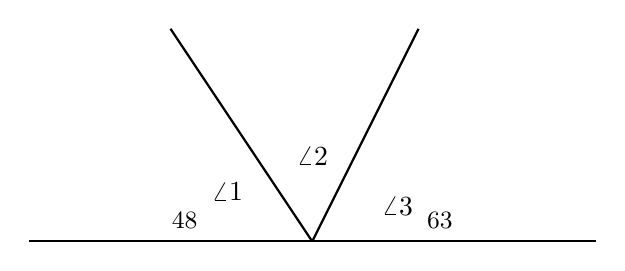
\begin{tikzpicture}[scale=0.9]
  \draw[thick] (-4,0) -- (4,0);
  \draw[thick] (0,0) -- (-2,3);
  \draw[thick] (0,0) -- (1.5,3);
  \node at (-1.2,0.7) {$\angle 1$};
  \node at (0,1.2) {$\angle 2$};
  \node at (1.2,0.5) {$\angle 3$};
  \node at (-1.8,0.3) {\small $48°$};
  \node at (1.8,0.3) {\small $63°$};
\end{tikzpicture}
\end{center}
\end{questionText}
\choiceA{$59°$}
\choiceB{$69°$}
\choiceC{$79°$}
\choiceD{$111°$}
\correctAnswer{B}
\explanation{Angles on a straight line sum to $180°$: $48° + \angle 2 + 63° = 180°$. Combine: $\angle 2 + 111° = 180°$. Subtract: $\angle 2 = 69°$.}
\end{practiceQuestion}

\begin{practiceQuestion}{m-6-6-q24}{gmc}
\begin{questionText}
In the triangle below, an exterior angle is formed at vertex $C$. Find the measure of the exterior angle.

\begin{center}
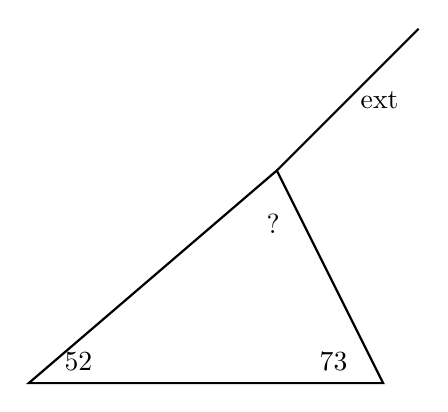
\begin{tikzpicture}[scale=0.9]
  \coordinate (A) at (0,0);
  \coordinate (B) at (5,0);
  \coordinate (C) at (3.5,3);
  \draw[thick] (A) -- (B) -- (C) -- cycle;
  % Exterior angle at C
  \draw[thick] (C) -- (5.5,5);
  % Interior angles
  \node at (0.7,0.3) {$52°$};
  \node at (4.3,0.3) {$73°$};
  \node at (3.45,2.25) {$?$};
  % Exterior angle label
  \node at (4.95,4.0) {ext};
\end{tikzpicture}
\end{center}
\end{questionText}
\choiceA{$55°$}
\choiceB{$107°$}
\choiceC{$125°$}
\choiceD{$180°$}
\correctAnswer{C}
\explanation{The interior angle at $C$ is $180° - 52° - 73° = 55°$. The exterior angle is supplementary to the interior angle at $C$: $180° - 55° = 125°$. Alternatively, by the exterior angle theorem: $52° + 73° = 125°$.}
\end{practiceQuestion}

% --- Graphical SA Questions (3) ---

\begin{practiceQuestion}{m-6-6-q25}{gsa}
\begin{questionText}
In the diagram, two parallel lines $\ell_1$ and $\ell_2$ are cut by a transversal $t$. Find the values of $a$ and $b$.

\begin{center}
\begin{tikzpicture}[scale=0.8]
  % Parallel lines
  \draw[thick] (-3,2) -- (4,2) node[right] {$\ell_1$};
  \draw[thick] (-3,-1) -- (4,-1) node[right] {$\ell_2$};
  % Transversal
  \draw[thick] (-1,3.5) -- (2,-2.5) node[right] {$t$};
  % Angle labels
  \node at (1.2,2.4) {$a°$};
  \node at (-0.8,1.6) {$115°$};
  \node at (1.8,-0.5) {$b°$};
\end{tikzpicture}
\end{center}
\end{questionText}
\correctAnswer{$a = 115°$, $b = 115°$}
\explanation{The $115°$ angle and angle $a$ are vertical angles at the top intersection, so $a = 115°$. Angle $b$ is corresponding to angle $a$ on the lower parallel line, so $b = 115°$.}
\end{practiceQuestion}

\begin{practiceQuestion}{m-6-6-q26}{gsa}
\begin{questionText}
In the figure, two straight lines intersect at point $O$. A ray $OC$ divides one of the angles into $p°$ and $35°$ as shown. The line from lower-left to upper-right makes a $59°$ angle with the horizontal. Find the values of $p$ and $q$.

\begin{center}
\begin{tikzpicture}[scale=0.9]
  \draw[thick] (-3,0) -- (3,0);
  \draw[thick] (-1.5,-2.5) -- (1.5,2.5);
  \draw[thick] (0,0) -- (2.5,1.8);
  % Labels
  \node at (1.8,0.4) {$p°$};
  \node at (1.4,1.3) {$35°$};
  \node at (-1.3,-0.7) {$q°$};
  \node at (0,-0.3) {$O$};
\end{tikzpicture}
\end{center}
\end{questionText}
\correctAnswer{$p = 24°$, $q = 59°$}
\explanation{The ray $OC$ divides the $59°$ angle between the horizontal and the upward line into $p°$ and $35°$. So $p + 35 = 59$, giving $p = 24°$. Angle $q$ is vertically opposite to the full $59°$ angle, so $q = 59°$.}
\end{practiceQuestion}

\begin{practiceQuestion}{m-6-6-q27}{gsa}
\begin{questionText}
In the diagram, $\triangle ABC$ is shown with an exterior angle at $B$. $\angle A = (3x + 5)°$ and $\angle C = (2x + 15)°$. The exterior angle at $B$ is $(7x - 10)°$. Find $x$ and all angle measures.

\begin{center}
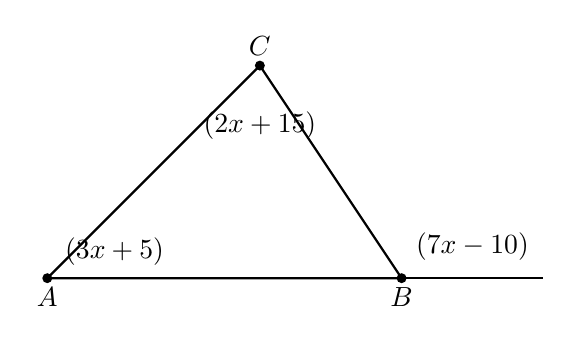
\begin{tikzpicture}[scale=0.9]
  \coordinate (A) at (0,0);
  \coordinate (B) at (5,0);
  \coordinate (C) at (3,3);
  \draw[thick] (A) -- (B) -- (C) -- cycle;
  % Exterior angle at B
  \draw[thick] (B) -- (7,0);
  % Labels
  \node at (0.95,0.38) {$(3x+5)°$};
  \node at (3.0,2.15) {$(2x+15)°$};
  \node at (6.0,0.45) {$(7x-10)°$};
  \fill (A) circle (2pt) node[below] {$A$};
  \fill (B) circle (2pt) node[below] {$B$};
  \fill (C) circle (2pt) node[above] {$C$};
\end{tikzpicture}
\end{center}
\end{questionText}
\correctAnswer{$x = 15$; $\angle A = 50°$, $\angle C = 45°$, $\angle B = 85°$, exterior angle $= 95°$}
\explanation{By the exterior angle theorem, the exterior angle equals the sum of the two non-adjacent interior angles: $7x - 10 = (3x + 5) + (2x + 15)$. Simplify: $7x - 10 = 5x + 20$. Subtract $5x$: $2x - 10 = 20$. Add $10$: $2x = 30$. Divide: $x = 15$. Then $\angle A = 3(15) + 5 = 50°$, $\angle C = 2(15) + 15 = 45°$. Interior $\angle B = 180° - 50° - 45° = 85°$. Exterior angle $= 7(15) - 10 = 95°$. Verify: $50 + 45 = 95$ \checkmark.}
\end{practiceQuestion}
